\chapter{Resultats}
\label{chap:Resultats}

  Per tal de validar que el sistema funciona, s'ha provat de fer un joc senzill amb ell, en aquest cas, un clon del Tetris.
  
  El Tetris és un joc creat el 1984, de mecàniques similars a un puzle i molt conegut arreu del món. La seva simplicitat i la seva fama el fan ideal com a exercici de programació. En podem veure una imatge a la figura \ref{fig:ImatgeTetris}.
  
  \begin{figure}
    \centering
    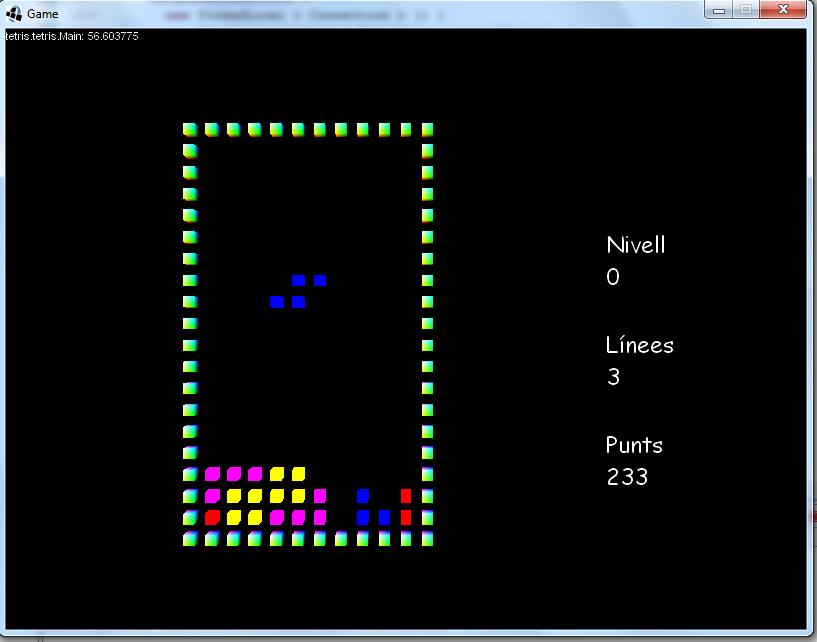
\includegraphics[width=0.5\linewidth]{./img/ImatgeTetris.png}
    \caption{Captura de pantalla del joc final \label{fig:ImatgeTetris}}
  \end{figure}
  
  Les mecàniques del Tetris són molt senzilles: distingim dues entitats bàsiques, el taulell i la peça. La peça cau des de la part superior del taulell, i el jugador pot modificar-ne la trajectòria i girar-la. Un cop la peça no pot descendir més, aquesta queda fixada al taulell i apareix una altra peça a la part superior. Si no pot aparèixer aquesta peça, el joc finalitza. En fixar una peça, pot ser que s'ocupi una línia sencera, en aquest cas s'elimina la línia i es beneficia al jugador amb un seguit de punts.

  En aquest capítol farem primer un repàs dels elements de Quadriga que s'han creat per programar el Tetris, seguidament es farà un cop d'ull a uns elements \"{}estàndard\"{} que s'han creat per tal d'ajudar-ne al desenvolupament. Finalment es farà un anàlisi sobre els objectius de disseny, punt per punt.
  
  \section{Elements propis del Tetris}

    Per tal de veure visualment com està muntat aquest Tetris, s'ha fet un diagrama semblant a l'UML de la seva estructura a la figura \ref{fig:TetrisEntitats}. També s'ha confeccionat una llegenda per entendre-ho millor, que es pot veure a la figura \ref{fig:GuiaDiagramaQuadriga}.

    \begin{figure}
      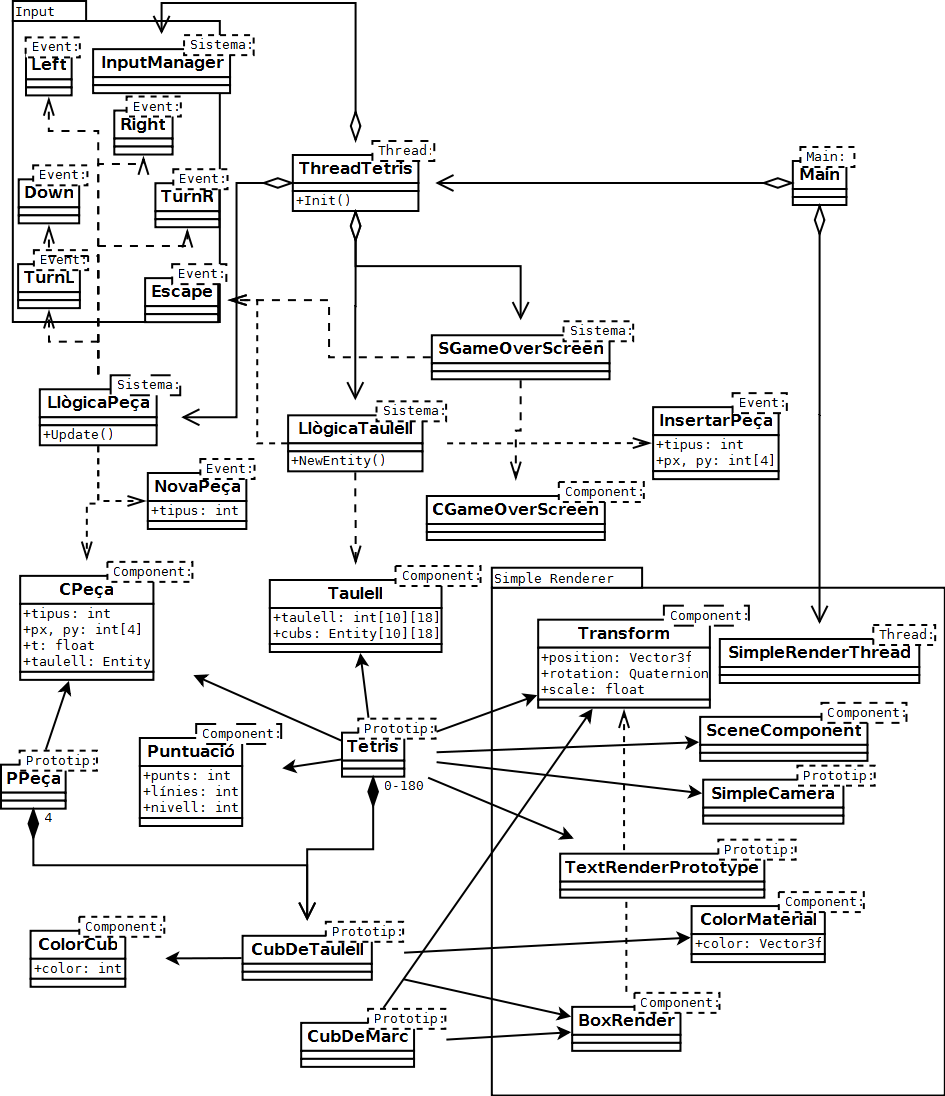
\includegraphics[width=1\linewidth]{./img/TetrisEntitats.png}
      \caption{Esquema dels elements que formen el Tetris \label{fig:TetrisEntitats}}
    \end{figure}

    \begin{figure}
      \centering
      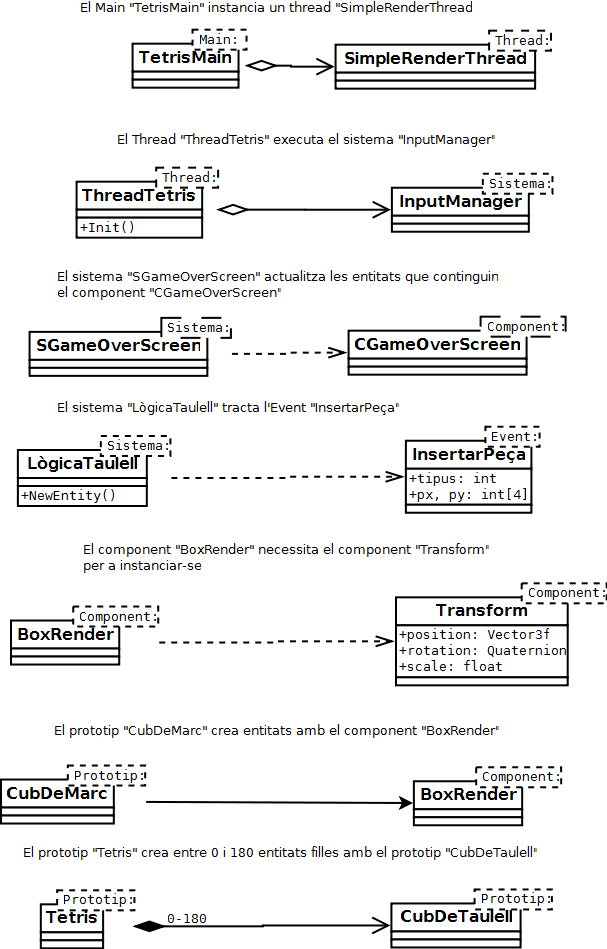
\includegraphics[width=0.7\linewidth]{./img/GuiaDiagramaQuadriga.png}
      \caption{Llegenda \label{fig:GuiaDiagramaQuadriga}}
    \end{figure}

    \subsection{Entitats / Prototips}
      
      \begin{itemize}
        \item {\bf Tetris}
          Representa l'estat actual del taulell de joc, amb els cubs posats, així com també conté informació sobre el nivell actual, els punts i les línies aconseguides pel jugador.
          
        \item {\bf Peça}
          Representa la peça que el jugador ha de col·locar en cada moment. Seria el més semblant a l'Avatar del jugador.
          
        \item {\bf CubDeMarc}
          Representa cada un dels cubs que fan de marc del taulell de joc.
          
        \item {\bf CubDeTaulell}
          Representen els cubs interiors del taulell, tant els col·locats com els que la peça actual aporta. Es diferencien dels anteriors ja que aquests han de tenir un color diferent depenent de la peça.
          
      \end{itemize}

    \subsection{Components}

      \begin{itemize}
        \item {\bf Taulell}
          Guarda informació de quines caselles del taulell estan ocupades per un cub, i en guarda una referència per eliminar-los o moure'ls quan el jugador completa una línia.
          
        \item {\bf Puntuació}
          Guarda informació sobre el nivell, les línies completades i la puntuació feta.
          
        \item {\bf Peça}
          Guarda informació sobre la forma i posició de la peça que actualment cau.
          
        \item {\bf ColorCub}
          Guarda informació sobre el color d'un cub.
          
        \item {\bf GameOverScreen}
          Representa la pantalla final, quan el jugador s'ha rendit o ha perdut.
          
      \end{itemize}

    \subsection{Events}

      \begin{itemize}
        \item {\bf NovaPeça}
          Es crea una nova peça, ja sigui per que s'inicia el joc o s'ha col·locat l'anterior. Aporta informació sobre quin tipus de peça s'ha de crear.
          
        \item {\bf InserirPeça}
          La peça ha arribat a sota i s'ha d'inserir al taulell.
          
        \item {\bf Left, Right, Down, TurnL, TurnR}
          El jugador ha donat instruccions per moure la peça o girar-la.
          
        \item {\bf Escape}
          El jugador ha premut la tecla d'escapament, volent finalitzar el joc o programa.
          
      \end{itemize}

    \subsection{Sistemes}

      \begin{itemize}
        \item {\bf LògicaTaulell}
          Controla la inserció de peces, l'acumulació de punts i si s'han completat línies, augmentant el nivell si s'escau.
          
        \item {\bf LògicaPeça}
          Controla que una peça es mogui segons les ordres del jugador i caigui a una velocitat donada pel nivell actual. També comprova si ha arribat al final i cal inserir-la.
          
        \item {\bf GameOverScreen}
          Un cop el jugador ha acabat la partida, en mostra la puntuació i espera que el jugador doni ordres de tancar el programa.
          
        \item {\bf InputManager}
          Vigila quin input dona el jugador i crea els events corresponents.
          
      \end{itemize}
      
    \subsection{Threads}
    
      \begin{itemize}
        \item {\bf ThreadTetris}
          Inicialitza el joc i executa els 4 sistemes anteriors.
          
      \end{itemize}
    
  \section{Llibreria SimpleRender}

    \subsection{Entitats / Prototips}

      \begin{itemize}
        \item {\bf TextRenderer}
          Renderitza un text donada una {\em Font}, una posició i un {\em String}.
      \end{itemize}


    \subsection{Components}

      \begin{itemize}
        \item {\bf Transform}
          Guarda informació sobre la translació, rotació i escala d'una entitat.
          
        \item {\bf SceneComponent}
          Marca un objecte com a arrel de l'escena.
          
        \item {\bf SimpleCamera}
          Guarda informació sobre la càmera de l'escena.
          
        \item {\bf ColorMaterial}
          L'objecte es renderitza amb un material de color pla.
          
        \item {\bf BoxRender}
          L'objecte es renderitza com una caixa.
          
      \end{itemize}
      
    \subsection{Threads}
    
      \begin{itemize}
        \item {\bf SimpleRenderThread}
          Renderitza tots els objectes de l'escena que contenen algun component \"{}renderitzable\"{} com {\em BoxRender}.
          
      \end{itemize}
      
\section{Objectius de disseny}

  S'analitza, punt per punt, si s'han complert els objectius de disseny del programa.
    
  \begin{figure}
    \centering
    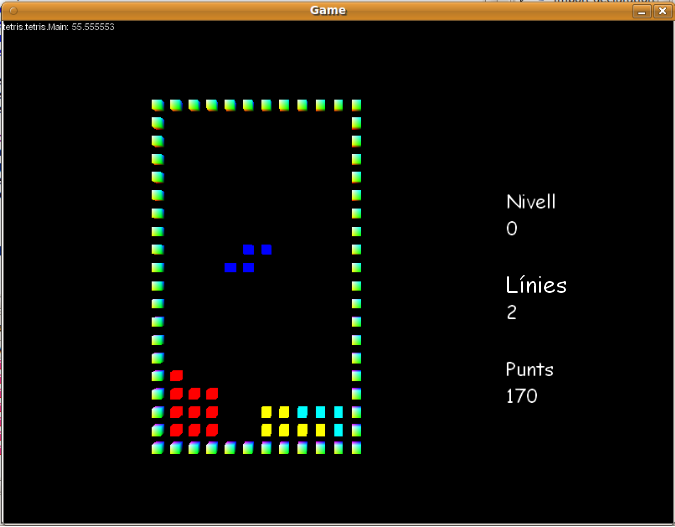
\includegraphics[width=0.5\linewidth]{./img/ImatgeUbuntu.png}
    \caption{Captura de pantalla del joc sobre Ubuntu \label{fig:ImatgeUbuntu}}
  \end{figure}

  \begin{itemize}
    \item {\bf Open Source} \hfill \\
      El codi es pot trobar a \url{https://code.google.com/p/quadriga/} sota llicència {\bf GNU Lesser GPL}.
      
    \item {\bf Independent} \hfill \\
      En l'exemple s'usen unes quantes llibreries Java per implementar aspectes importants del joc. {\em OpenGL} i l'{\em input} del jugador s'obtenen a partir de {\bf LWJGL}. Per fer-les servir des de {\em Quadriga} cal emprar {\em Components} que anomenaríem "estàndard" sota el paquet {\em cat.quadriga.base}. Fer aquests components no és senzill, però es podrien substituir els sistemes si es volgués fer l'esforç sense masses problemes.
      
    \item {\bf Multi-plataforma de forma nativa} \hfill \\
      Com es veu a la figura \ref{fig:ImatgeUbuntu}, el joc corre sobre {\em Ubuntu} sense cap diferència. El codi Java i Quadriga no s'han tocat, però si que cal fer una petita modificació a l'hora de crear l'executable, doncs {\em OpenGL} necessita accedir a llibreries natives que són diferents en cada plataforma.
      
    \item {\bf Permetre un desenvolupament ràpid un cop estiguin fets els components bàsics} \hfill \\
      El codi final són 2 arxius, un de lògica de unes 800 línies i un altre de input de 65. És de fet quasi més llarg fer el disseny que no implementar-lo.
      
      Addicionalment s'ha provat d'afegir funcionalitat. En vint minuts s'ha aconseguit inserir una guia per indicar la peça següent a caure. En total s'han afegit 140 línies (afegir el component, prototip i sistema que controlin la peça següent), de les quals pràcticament totes són una còpia de codi ja fet, i s'han hagut de modificar 3 punts del joc, on s'instanciava una nova peça per tal de fer que agafés el tipus de peça que hi havia guardat. Veure figura \ref{fig:ImatgePecaSeguent}.
      
    \item {\bf Fàcilment paral·lelitzable} \hfill \\
      Actualment el programa conté una opció de fer córrer cada {\em Thread} en paral·lel, però l'opció teòricament òptima de paral·lelitzar l'actualització de cada entitat sobre cada sistema (aconseguint una paral·lelització no sobre el nombre de threads, sinó sobre el nombre d'entitats) no s'ha implementat.
  \end{itemize}
    
  \begin{figure}
    \centering
    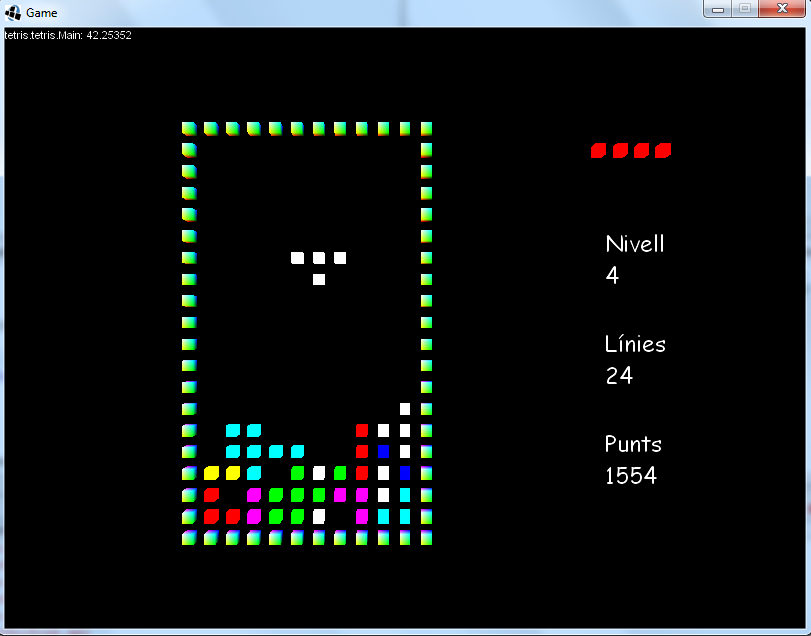
\includegraphics[width=0.5\linewidth]{./img/ImatgePecaSeguent.png}
    \caption{Captura de pantalla del joc amb modificacions \label{fig:ImatgePecaSeguent}}
  \end{figure}

  Per tal de validar els resultats, s'ha considerat que el fet de poder programar-hi un joc consisteix una prova força complerta de que el projecte funciona. S'ha demostrat que el joc es pot ampliar fàcilment. Ara es proposaran alguns dissenys de millora:
  
  \begin{itemize}
    \item {\bf Multi-jugador a pantalla dividida:} Per tal d'implementar aquesta millora, cal duplicar les entitats principals: tenir 2 sistemes i 2 peces. També cal ampliar els events d'ordres del jugador tal que aportin informació de quin jugador l'ha feta, i que les funcions que responen a aquests events actuïn sobre la peça adequada.
    
    \item {\bf Multi-jugador en xarxa:} Aquesta ampliació és en part més complexa que l'anterior, ja que implica crear un mòdul de xarxa. Un cop creat aquest mòdul, les modificacions al programa Quadriga són mínimes, ja que només cal fer que els events que el jugador local crea s'enviïn al jugador remot, i fer que els events remots es tradueixin als events locals.
    
    \item {\bf Crear un fons de pantalla més estètic:} Cal crear un component i una entitat que controlin el fons de pantalla, així com ampliar la llibreria gràfica. Tot això aniria associat a la llibreria estàndard de Quadriga i les modificacions des del nucli de la lògica serien mínimes.
    
    \item {\em Crear un menú principal amb pantalla de rècords:} Caldria crear una màquina d'estats que implementés aquest menú. La llibreria estàndard ja incorpora utilitats per renderitzar qualsevol text en {\bf Unicode}. Addicionalment, es podria afegir funcionalitat per guardar l'estat de la base de dades i així mantenir els rècords entre partides.
  \end{itemize}

  